\documentclass[11pt,preprint]{elsarticle}

\usepackage{lmodern}
%%%% My spacing
\usepackage{setspace}
\setstretch{1.2}
\DeclareMathSizes{12}{14}{10}{10}

% Wrap around which gives all figures included the [H] command, or places it "here". This can be tedious to code in Rmarkdown.
\usepackage{float}
\let\origfigure\figure
\let\endorigfigure\endfigure
\renewenvironment{figure}[1][2] {
    \expandafter\origfigure\expandafter[H]
} {
    \endorigfigure
}

\let\origtable\table
\let\endorigtable\endtable
\renewenvironment{table}[1][2] {
    \expandafter\origtable\expandafter[H]
} {
    \endorigtable
}


\usepackage{ifxetex,ifluatex}
\usepackage{fixltx2e} % provides \textsubscript
\ifnum 0\ifxetex 1\fi\ifluatex 1\fi=0 % if pdftex
  \usepackage[T1]{fontenc}
  \usepackage[utf8]{inputenc}
\else % if luatex or xelatex
  \ifxetex
    \usepackage{mathspec}
    \usepackage{xltxtra,xunicode}
  \else
    \usepackage{fontspec}
  \fi
  \defaultfontfeatures{Mapping=tex-text,Scale=MatchLowercase}
  \newcommand{\euro}{€}
\fi

\usepackage{amssymb, amsmath, amsthm, amsfonts}

\def\bibsection{\section*{References}} %%% Make "References" appear before bibliography


\usepackage[numbers]{natbib}

\usepackage{longtable}
\usepackage[margin=2.3cm,bottom=2cm,top=2.5cm, includefoot]{geometry}
\usepackage{fancyhdr}
\usepackage[bottom, hang, flushmargin]{footmisc}
\usepackage{graphicx}
\numberwithin{equation}{section}
\numberwithin{figure}{section}
\numberwithin{table}{section}
\setlength{\parindent}{0cm}
\setlength{\parskip}{1.3ex plus 0.5ex minus 0.3ex}
\usepackage{textcomp}
\renewcommand{\headrulewidth}{0.2pt}
\renewcommand{\footrulewidth}{0.3pt}

\usepackage{array}
\newcolumntype{x}[1]{>{\centering\arraybackslash\hspace{0pt}}p{#1}}

%%%%  Remove the "preprint submitted to" part. Don't worry about this either, it just looks better without it:

 \def\tightlist{} % This allows for subbullets!

\usepackage{hyperref}
\hypersetup{breaklinks=true,
            bookmarks=true,
            colorlinks=true,
            citecolor=blue,
            urlcolor=blue,
            linkcolor=blue,
            pdfborder={0 0 0}}


% The following packages allow huxtable to work:
\usepackage{siunitx}
\usepackage{multirow}
\usepackage{hhline}
\usepackage{calc}
\usepackage{tabularx}
\usepackage{booktabs}
\usepackage{caption}


\newenvironment{columns}[1][]{}{}

\newenvironment{column}[1]{\begin{minipage}{#1}\ignorespaces}{%
\end{minipage}
\ifhmode\unskip\fi
\aftergroup\useignorespacesandallpars}

\def\useignorespacesandallpars#1\ignorespaces\fi{%
#1\fi\ignorespacesandallpars}

\makeatletter
\def\ignorespacesandallpars{%
  \@ifnextchar\par
    {\expandafter\ignorespacesandallpars\@gobble}%
    {}%
}
\makeatother


% definitions for citeproc citations
\NewDocumentCommand\citeproctext{}{}
\NewDocumentCommand\citeproc{mm}{%
\href{\#cite.\detokenize{#1}}{#2}\nocite{#1}}

\makeatletter
% allow citations to break across lines
\let\@cite@ofmt\@firstofone
% avoid brackets around text for \cite:
\def\@biblabel#1{}
\def\@cite#1#2{{#1\if@tempswa , #2\fi}}
\makeatother
\newlength{\cslhangindent}
\setlength{\cslhangindent}{1.5em}
\newlength{\csllabelwidth}
\setlength{\csllabelwidth}{3em}
\newenvironment{CSLReferences}[2] % #1 hanging-indent, #2 entry-spacing
{\begin{list}{}{%
	\setlength{\itemindent}{0pt}
	\setlength{\leftmargin}{0pt}
	\setlength{\parsep}{0pt}
	% turn on hanging indent if param 1 is 1
	\ifodd #1
	\setlength{\leftmargin}{\cslhangindent}
	\setlength{\itemindent}{-1\cslhangindent}
	\fi
	% set entry spacing
	\setlength{\itemsep}{#2\baselineskip}}}
{\end{list}}

\usepackage{calc}
\newcommand{\CSLBlock}[1]{\hfill\break\parbox[t]{\linewidth}{\strut\ignorespaces#1\strut}}
\newcommand{\CSLLeftMargin}[1]{\parbox[t]{\csllabelwidth}{\strut#1\strut}}
\newcommand{\CSLRightInline}[1]{\parbox[t]{\linewidth - \csllabelwidth}{\strut#1\strut}}
\newcommand{\CSLIndent}[1]{\hspace{\cslhangindent}#1}


\urlstyle{same}  % don't use monospace font for urls
\setlength{\parindent}{0pt}
\setlength{\parskip}{6pt plus 2pt minus 1pt}
\setlength{\emergencystretch}{3em}  % prevent overfull lines
\setcounter{secnumdepth}{5}

%%% Use protect on footnotes to avoid problems with footnotes in titles
\let\rmarkdownfootnote\footnote%
\def\footnote{\protect\rmarkdownfootnote}
\IfFileExists{upquote.sty}{\usepackage{upquote}}{}

%%% Include extra packages specified by user

%%% Hard setting column skips for reports - this ensures greater consistency and control over the length settings in the document.
%% page layout
%% paragraphs
\setlength{\baselineskip}{12pt plus 0pt minus 0pt}
\setlength{\parskip}{12pt plus 0pt minus 0pt}
\setlength{\parindent}{0pt plus 0pt minus 0pt}
%% floats
\setlength{\floatsep}{12pt plus 0 pt minus 0pt}
\setlength{\textfloatsep}{20pt plus 0pt minus 0pt}
\setlength{\intextsep}{14pt plus 0pt minus 0pt}
\setlength{\dbltextfloatsep}{20pt plus 0pt minus 0pt}
\setlength{\dblfloatsep}{14pt plus 0pt minus 0pt}
%% maths
\setlength{\abovedisplayskip}{12pt plus 0pt minus 0pt}
\setlength{\belowdisplayskip}{12pt plus 0pt minus 0pt}
%% lists
\setlength{\topsep}{10pt plus 0pt minus 0pt}
\setlength{\partopsep}{3pt plus 0pt minus 0pt}
\setlength{\itemsep}{5pt plus 0pt minus 0pt}
\setlength{\labelsep}{8mm plus 0mm minus 0mm}
\setlength{\parsep}{\the\parskip}
\setlength{\listparindent}{\the\parindent}
%% verbatim
\setlength{\fboxsep}{5pt plus 0pt minus 0pt}



\begin{document}



\begin{frontmatter}  %

\title{Local Coffee Report}

% Set to FALSE if wanting to remove title (for submission)












\vspace{1cm}





\vspace{0.5cm}

\end{frontmatter}

\setcounter{footnote}{0}



%________________________
% Header and Footers
%%%%%%%%%%%%%%%%%%%%%%%%%%%%%%%%%
\pagestyle{fancy}
\chead{}
\rhead{}
\lfoot{}
\rfoot{\footnotesize Page \thepage}
\lhead{}
%\rfoot{\footnotesize Page \thepage } % "e.g. Page 2"
\cfoot{}

%\setlength\headheight{30pt}
%%%%%%%%%%%%%%%%%%%%%%%%%%%%%%%%%
%________________________

\headsep 35pt % So that header does not go over title




\section{Loading and cleaning data}\label{loading-and-cleaning-data}

First, I want to inspect the data to check its format and how messy it
is

In order to handle uppercase column names and load the coffee data the
load\_data function is used:

Additional issue with the data: the dates are in (Mon-YY) format; the
country column has a typo where it reads ``United States and Floyd'';
and there are missing values in the roast column. Therefore:

\section{Cost and rating}\label{cost-and-rating}

First, we will investigate the relationship between cost and rating by
the location of the roaster. As rating is a discrete variable, we will
use a boxplot.

\begin{figure}[H]

{\centering 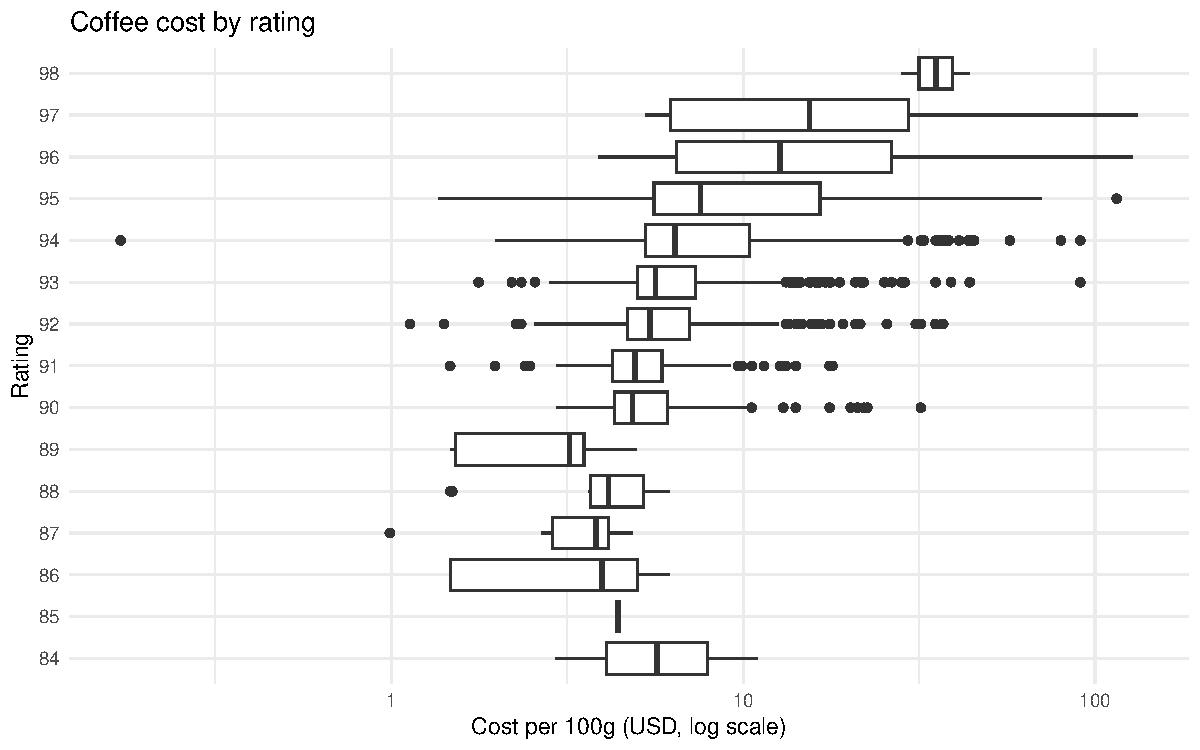
\includegraphics{22921893Question1_files/figure-latex/unnamed-chunk-4-1} 

}

\caption{Cost and rating.}\label{fig:unnamed-chunk-4}
\end{figure}

The plot displays an upward trend, where higher ratings cluster at a
higher cost. The mid-range of ratings overlap significantly, with long
tails in both directions. As the United States (n = 1332) and Taiwan (n
= 549) are the countries which roast the most coffee beans, they are the
predominant countries in the data. To visualise the cost distribution of
these countries the following functions are run:

\begin{figure}[H]

{\centering 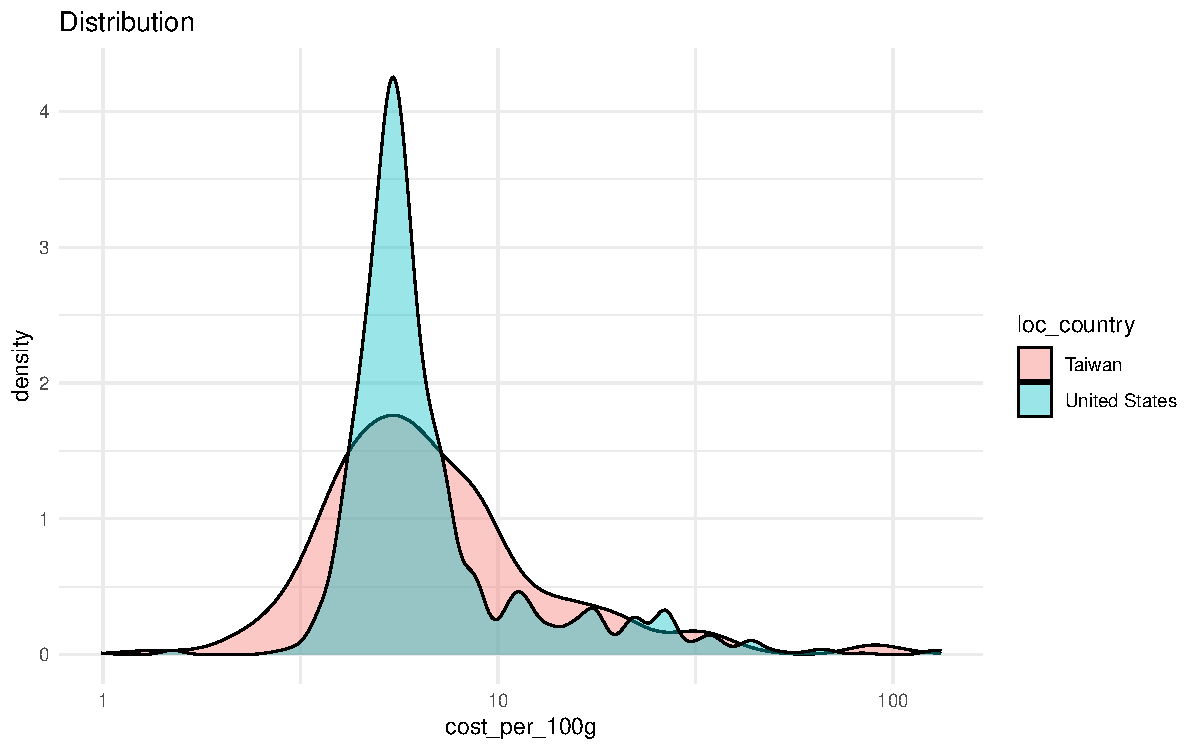
\includegraphics{22921893Question1_files/figure-latex/unnamed-chunk-5-1} 

}

\caption{The US and Taiwan.}\label{fig:unnamed-chunk-5}
\end{figure}

As the goal should ultimately be to find good value coffee, I define a
value metric as rating divided by cost per 100g. This tells the buyer
how much rating she is getting per dollar spent. The function also
filters coffees with implausibly low cost.

After removing the two implausible entries, the value metric now ranges
from 0.7 to 81.4, with a mean of 15.4 and a median of 16.0. Coffee costs
are skewed right, indicating most coffees are reasonably priced with a
few expensive coffees also present in the sample. In contrast, ratings
are tightly clustered, ranging between 84 and 98.

\begin{longtable}[]{@{}lrrrrr@{}}
\caption{Descriptive statistics}\tabularnewline
\toprule\noalign{}
variable & mean & median & sd & min & max \\
\midrule\noalign{}
\endfirsthead
\toprule\noalign{}
variable & mean & median & sd & min & max \\
\midrule\noalign{}
\endhead
\bottomrule\noalign{}
\endlastfoot
cost\_per\_100g & 9.1 & 5.9 & 10.3 & 1.1 & 132.3 \\
rating & 93.1 & 93.0 & 1.6 & 84.0 & 98.0 \\
value & 15.4 & 16.0 & 7.6 & 0.7 & 81.4 \\
\end{longtable}

The following table depicts the Top 10 roasters by median value.
Inclusion as a candidate for best value roaster requires at least 5
coffees. Mr.~Chao Coffee, El Gran Cafe, and Jackrabbit Java lead with
median values around 22-25. These roasters deliver substantially more
rating per dollar spent than the sample median of 16.0.

\begin{longtable}[]{@{}
  >{\raggedright\arraybackslash}p{(\linewidth - 8\tabcolsep) * \real{0.3676}}
  >{\raggedleft\arraybackslash}p{(\linewidth - 8\tabcolsep) * \real{0.0588}}
  >{\raggedleft\arraybackslash}p{(\linewidth - 8\tabcolsep) * \real{0.1765}}
  >{\raggedleft\arraybackslash}p{(\linewidth - 8\tabcolsep) * \real{0.2059}}
  >{\raggedleft\arraybackslash}p{(\linewidth - 8\tabcolsep) * \real{0.1912}}@{}}
\caption{Top 10 roasters by value (median)}\tabularnewline
\toprule\noalign{}
\begin{minipage}[b]{\linewidth}\raggedright
roaster
\end{minipage} & \begin{minipage}[b]{\linewidth}\raggedleft
n
\end{minipage} & \begin{minipage}[b]{\linewidth}\raggedleft
median\_cost
\end{minipage} & \begin{minipage}[b]{\linewidth}\raggedleft
median\_rating
\end{minipage} & \begin{minipage}[b]{\linewidth}\raggedleft
median\_value
\end{minipage} \\
\midrule\noalign{}
\endfirsthead
\toprule\noalign{}
\begin{minipage}[b]{\linewidth}\raggedright
roaster
\end{minipage} & \begin{minipage}[b]{\linewidth}\raggedleft
n
\end{minipage} & \begin{minipage}[b]{\linewidth}\raggedleft
median\_cost
\end{minipage} & \begin{minipage}[b]{\linewidth}\raggedleft
median\_rating
\end{minipage} & \begin{minipage}[b]{\linewidth}\raggedleft
median\_value
\end{minipage} \\
\midrule\noalign{}
\endhead
\bottomrule\noalign{}
\endlastfoot
Mr.~Chao Coffee & 5 & 3.67 & 92 & 24.80 \\
El Gran Cafe & 29 & 3.82 & 91 & 23.56 \\
Jackrabbit Java & 23 & 4.12 & 92 & 22.33 \\
Coffee By Design & 7 & 4.08 & 93 & 22.30 \\
Kakalove Cafe & 142 & 4.25 & 94 & 22.00 \\
Mystic Monk Coffee & 9 & 4.11 & 91 & 21.90 \\
Propeller Coffee & 10 & 4.32 & 93 & 21.67 \\
San Francisco Bay Coffee & 9 & 4.17 & 90 & 21.10 \\
Espresso Republic & 11 & 4.41 & 90 & 20.63 \\
Creation Food Co. & 5 & 4.51 & 91 & 19.96 \\
\end{longtable}

\section{\texorpdfstring{Indicators of good coffee
\label{Indicators of good coffee }}{Indicators of good coffee }}\label{indicators-of-good-coffee}

Per the practical instructions, the most important keywords that
Stelenbosch students have used as indicators of good coffee are: - sweet
- finish - mouthfeel - structure - aroma - chocolate - toned

Therefore, I first generate a new dataset, which includes a count of
these important keywords individually as well as a total column.

This new dataset is more complete, as it includes valuable information:
the frequency of keywords which Stellenbosch students regard as
desirable. This is valuable information, as it provides an indicator of
what qualities may make a coffee in Stellenbosch a best seller.

\section{Which roaster is the `best'?}\label{which-roaster-is-the-best}

To see whether the roasters with the best value also score well on
keyword indicators, I add the average keyword count per roaster to the
top 10 value rankings. This indicates there a tradeoff when choosing a
roaster to supply coffee. The roasters with the highest rating
(e.g.~Kakalove Cafe) are more expensive, and do not necessarily have a
higher frequency of desirable keywords. is Two roasters stand out in the
table as having a particularly high keyword average, Mystic Monk Coffee
and Creation Food Co.

\begin{longtable}[]{@{}
  >{\raggedright\arraybackslash}p{(\linewidth - 10\tabcolsep) * \real{0.2841}}
  >{\raggedleft\arraybackslash}p{(\linewidth - 10\tabcolsep) * \real{0.0455}}
  >{\raggedleft\arraybackslash}p{(\linewidth - 10\tabcolsep) * \real{0.1364}}
  >{\raggedleft\arraybackslash}p{(\linewidth - 10\tabcolsep) * \real{0.1591}}
  >{\raggedleft\arraybackslash}p{(\linewidth - 10\tabcolsep) * \real{0.1477}}
  >{\raggedleft\arraybackslash}p{(\linewidth - 10\tabcolsep) * \real{0.2273}}@{}}
\caption{Top 10 roasters by value, with average keywords}\tabularnewline
\toprule\noalign{}
\begin{minipage}[b]{\linewidth}\raggedright
roaster
\end{minipage} & \begin{minipage}[b]{\linewidth}\raggedleft
n
\end{minipage} & \begin{minipage}[b]{\linewidth}\raggedleft
median\_cost
\end{minipage} & \begin{minipage}[b]{\linewidth}\raggedleft
median\_rating
\end{minipage} & \begin{minipage}[b]{\linewidth}\raggedleft
median\_value
\end{minipage} & \begin{minipage}[b]{\linewidth}\raggedleft
total\_keywords\_mean
\end{minipage} \\
\midrule\noalign{}
\endfirsthead
\toprule\noalign{}
\begin{minipage}[b]{\linewidth}\raggedright
roaster
\end{minipage} & \begin{minipage}[b]{\linewidth}\raggedleft
n
\end{minipage} & \begin{minipage}[b]{\linewidth}\raggedleft
median\_cost
\end{minipage} & \begin{minipage}[b]{\linewidth}\raggedleft
median\_rating
\end{minipage} & \begin{minipage}[b]{\linewidth}\raggedleft
median\_value
\end{minipage} & \begin{minipage}[b]{\linewidth}\raggedleft
total\_keywords\_mean
\end{minipage} \\
\midrule\noalign{}
\endhead
\bottomrule\noalign{}
\endlastfoot
Mr.~Chao Coffee & 5 & 3.67 & 92 & 24.80 & 8.20 \\
El Gran Cafe & 29 & 3.82 & 91 & 23.56 & 8.59 \\
Jackrabbit Java & 23 & 4.12 & 92 & 22.33 & 8.65 \\
Coffee By Design & 7 & 4.08 & 93 & 22.30 & 9.29 \\
Kakalove Cafe & 142 & 4.25 & 94 & 22.00 & 8.61 \\
Mystic Monk Coffee & 9 & 4.11 & 91 & 21.90 & 11.33 \\
Propeller Coffee & 10 & 4.32 & 93 & 21.67 & 9.00 \\
San Francisco Bay Coffee & 9 & 4.17 & 90 & 21.10 & 9.11 \\
Espresso Republic & 11 & 4.41 & 90 & 20.63 & 9.36 \\
Creation Food Co. & 5 & 4.51 & 91 & 19.96 & 10.60 \\
\end{longtable}

The following plot depicts the trade-off when choosing a roaster to
supply coffee. As high-rating-roasters are often more expensive, and do
not necessarily have more desirable characteristics (as proxied by the
frequency of desirable words in the reviews). The following plot
displays the relationship between rating (mean) and cost (mean) for each
roasters. A clear positive relationship can be seen between rating and
cost. The colour corresponds to the mean frequency of desirable words
that these roasters have in their coffee (per the reviews). The three
roasters that most often have desirable words in their coffee's
descriptions are Mystic Monk Coffee, Creation Food Co., and Corvus
Coffee Roasters. Of these three, only two appeared in the top value
rankings: Mystic Monk Coffee and Creation Food Co.~Therefore, it is
contended these are the `best' roasters, as they provide provide great
value while having a high frequency of desirable keywords.

\begin{figure}[H]

{\centering 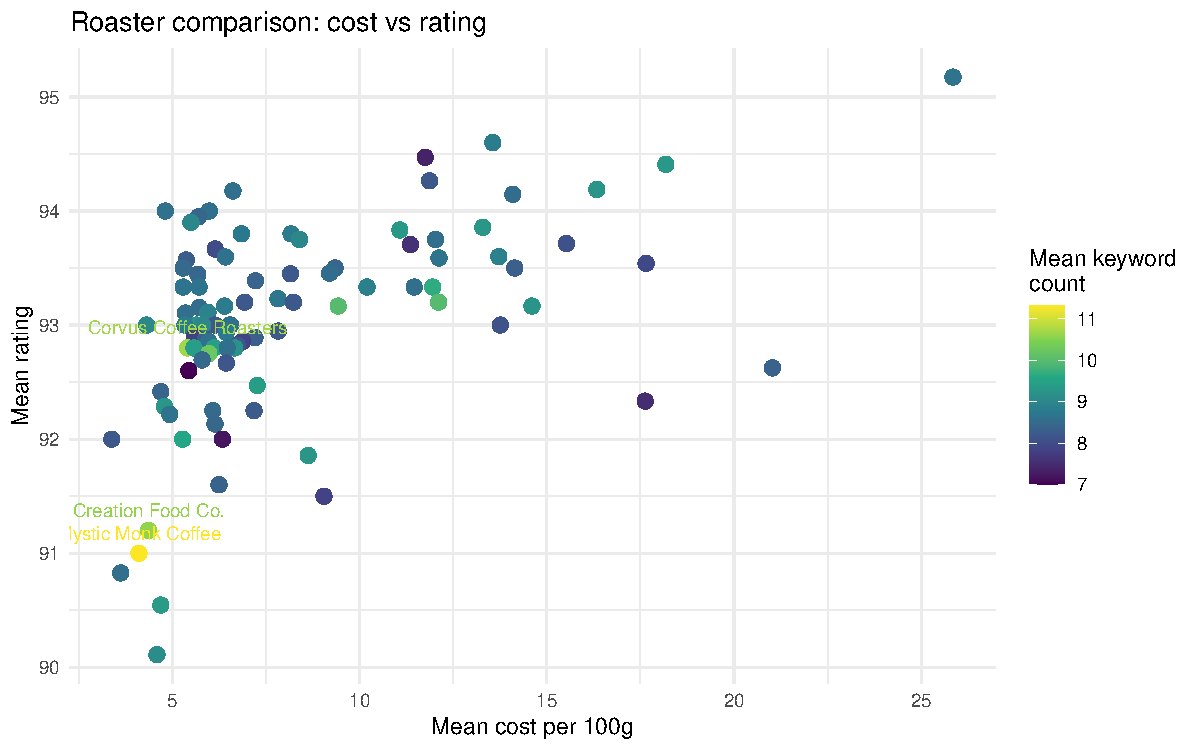
\includegraphics{22921893Question1_files/figure-latex/unnamed-chunk-11-1} 

}

\caption{Roaster Scatterplot.}\label{fig:unnamed-chunk-11}
\end{figure}

\bibliography{Tex/ref}





\end{document}
